\documentclass[a4,12pt]{article}
\usepackage{colortbl}
\usepackage{pgfplots}
\usepackage[margin=2cm]{geometry}
\pgfplotsset{compat=newest}
\begin{document}
\begin{table}
\footnotesize
\sffamily
\begin{center}
\begin{tabular}{ccccccccc}
Mean-Accuracy & \shortstack{LITETime \\ 0.7929} & \shortstack{InceptionTime \\ 0.7924} & \shortstack{Inception \\ 0.7807} & \shortstack{ROCKET \\ 0.7733} & \shortstack{LITE \\ 0.7694} & \shortstack{ResNet \\ 0.7491} & \shortstack{FCN \\ 0.7276} \\[1ex]
\shortstack{MMM4TSC \\ 0.7940} & \cellcolor[rgb]{0.8715,0.8623,0.857}\shortstack{\rule{0em}{3ex} 0.0011 \\ 16 / 0 / 19 \\ 0.7524} & \cellcolor[rgb]{0.8756,0.8602,0.8514}\shortstack{\rule{0em}{3ex} 0.0016 \\ 16 / 0 / 19 \\ 0.6330} & \cellcolor[rgb]{0.9383,0.8089,0.7412}\shortstack{\rule{0em}{3ex} 0.0133 \\ 19 / 0 / 16 \\ 0.2071} & \cellcolor[rgb]{0.9606,0.7625,0.668}\shortstack{\rule{0em}{3ex} 0.0207 \\ 20 / 0 / 15 \\ 0.2318} & \bfseries \cellcolor[rgb]{0.967,0.7357,0.6309}\shortstack{\rule{0em}{3ex} 0.0246 \\ 21 / 0 / 14 \\ 0.0371} & \bfseries \cellcolor[rgb]{0.9417,0.5464,0.4297}\shortstack{\rule{0em}{3ex} 0.0449 \\ 20 / 1 / 14 \\ 0.0078} & \bfseries \cellcolor[rgb]{0.8204,0.2868,0.2452}\shortstack{\rule{0em}{3ex} 0.0664 \\ 26 / 0 / 9 \\  $\leq$ 1e-04} & \shortstack{\rule{0em}{3ex} Mean-Difference \\ r$>$c / r=c / r$<$c \\ Wilcoxon p-value} \\[1ex]
\end{tabular}\\
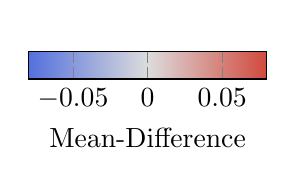
\begin{tikzpicture}[baseline=(current bounding box.center)]\begin{axis}[hide axis,scale only axis,width=0sp,height=0sp,colorbar horizontal,colorbar style={width=0.25\linewidth,colormap={cm}{rgb255(1)=(83,112,221) rgb255(2)=(220,220,220) rgb255(3)=(209,73,62)},colorbar horizontal,point meta min=-0.08,point meta max=0.08,colorbar/width=1.0em,scaled x ticks=false,xticklabel style={/pgf/number format/fixed,/pgf/number format/precision=3},xlabel={Mean-Difference},}] \addplot[draw=none] {0};\end{axis}\end{tikzpicture}\end{center}
\caption{[...] \textbf{If in bold, then p-value $<$ 0.05} [...]}
\end{table}
\end{document}
